\chapter{Diseño de Estructuras de Metal y Madera}

\begin{example}
  Se tiene una armadura con las siguientes dimensiones:
  \begin{itemize}
    \item $l=15m$
    \item $h\approx \frac{l}{10}$
    \item $W_{viva}= 400 kg/m^2$
    \item ancho de $1.5m$
    \item Acero A-36 ($F_y=2515kg/cm^2$)
  \end{itemize}
\end{example}

Super: la parte superior del puente
1.50-1.80m
contravientos: acero que son diagonales o verticales,
lamina acanalada, por debajo del concreto para que no se deformen en el plano vertical por el viento,
conexión: son cuadrados
Acero A50
Método elástico
Norma rfd
$\omega_{viva}=400$, $\omega_{losa}=152.2kg/m^2+25kg/m^2$, $\omega_{lamina}=602kg/m^2$, $\omega_{total}= 583.2kg/m^2$ b=1.5, 
\begin{align*}
    \omega = \omega_{por m^2}(1.5) = 879.8 \frac{kg}{m}\\
    P_{por nodo} = \frac{\omega(1)}{2} = 437.4kg
\end{align*}
Se multiplica los nodos por la cantidad de nodos (9):
$R_1=437.4\cdot 9=2187kg$ y $R_2=437.4\cdot 9=2187kg$
Por Pitágoras, la diagonal es:
\begin{equation*}
    D = \sqrt{2.1^2 + 0.5^2} = 2.32
\end{equation*}
si (2.32m)*22kg = 51.04kg
\begin{align*}
    &- 51.04(0.5) + By(1) - Bx(2.1) = 0\\
    &\sum F_x = 0\\
    &Ax - Bx = 0\implies Ax = \Delta x\\
    &\sum M = 0\\
    &51.04(0.5) - Ay(1)\\
    &- Ax(2.1) = 0\\
    &\sum Fy = 0\\
    &Ay + By - 51.04 = 0\\
    &Ay = 51.04 - By\\
    &51.04(0.5) -(51.04 - By) - By(2.1) = 0
\end{align*}
Tensión, compresión, cortante, flexo-compresión.

Armadura simple e isostática:

\begin{figure}[h!]
\centering
  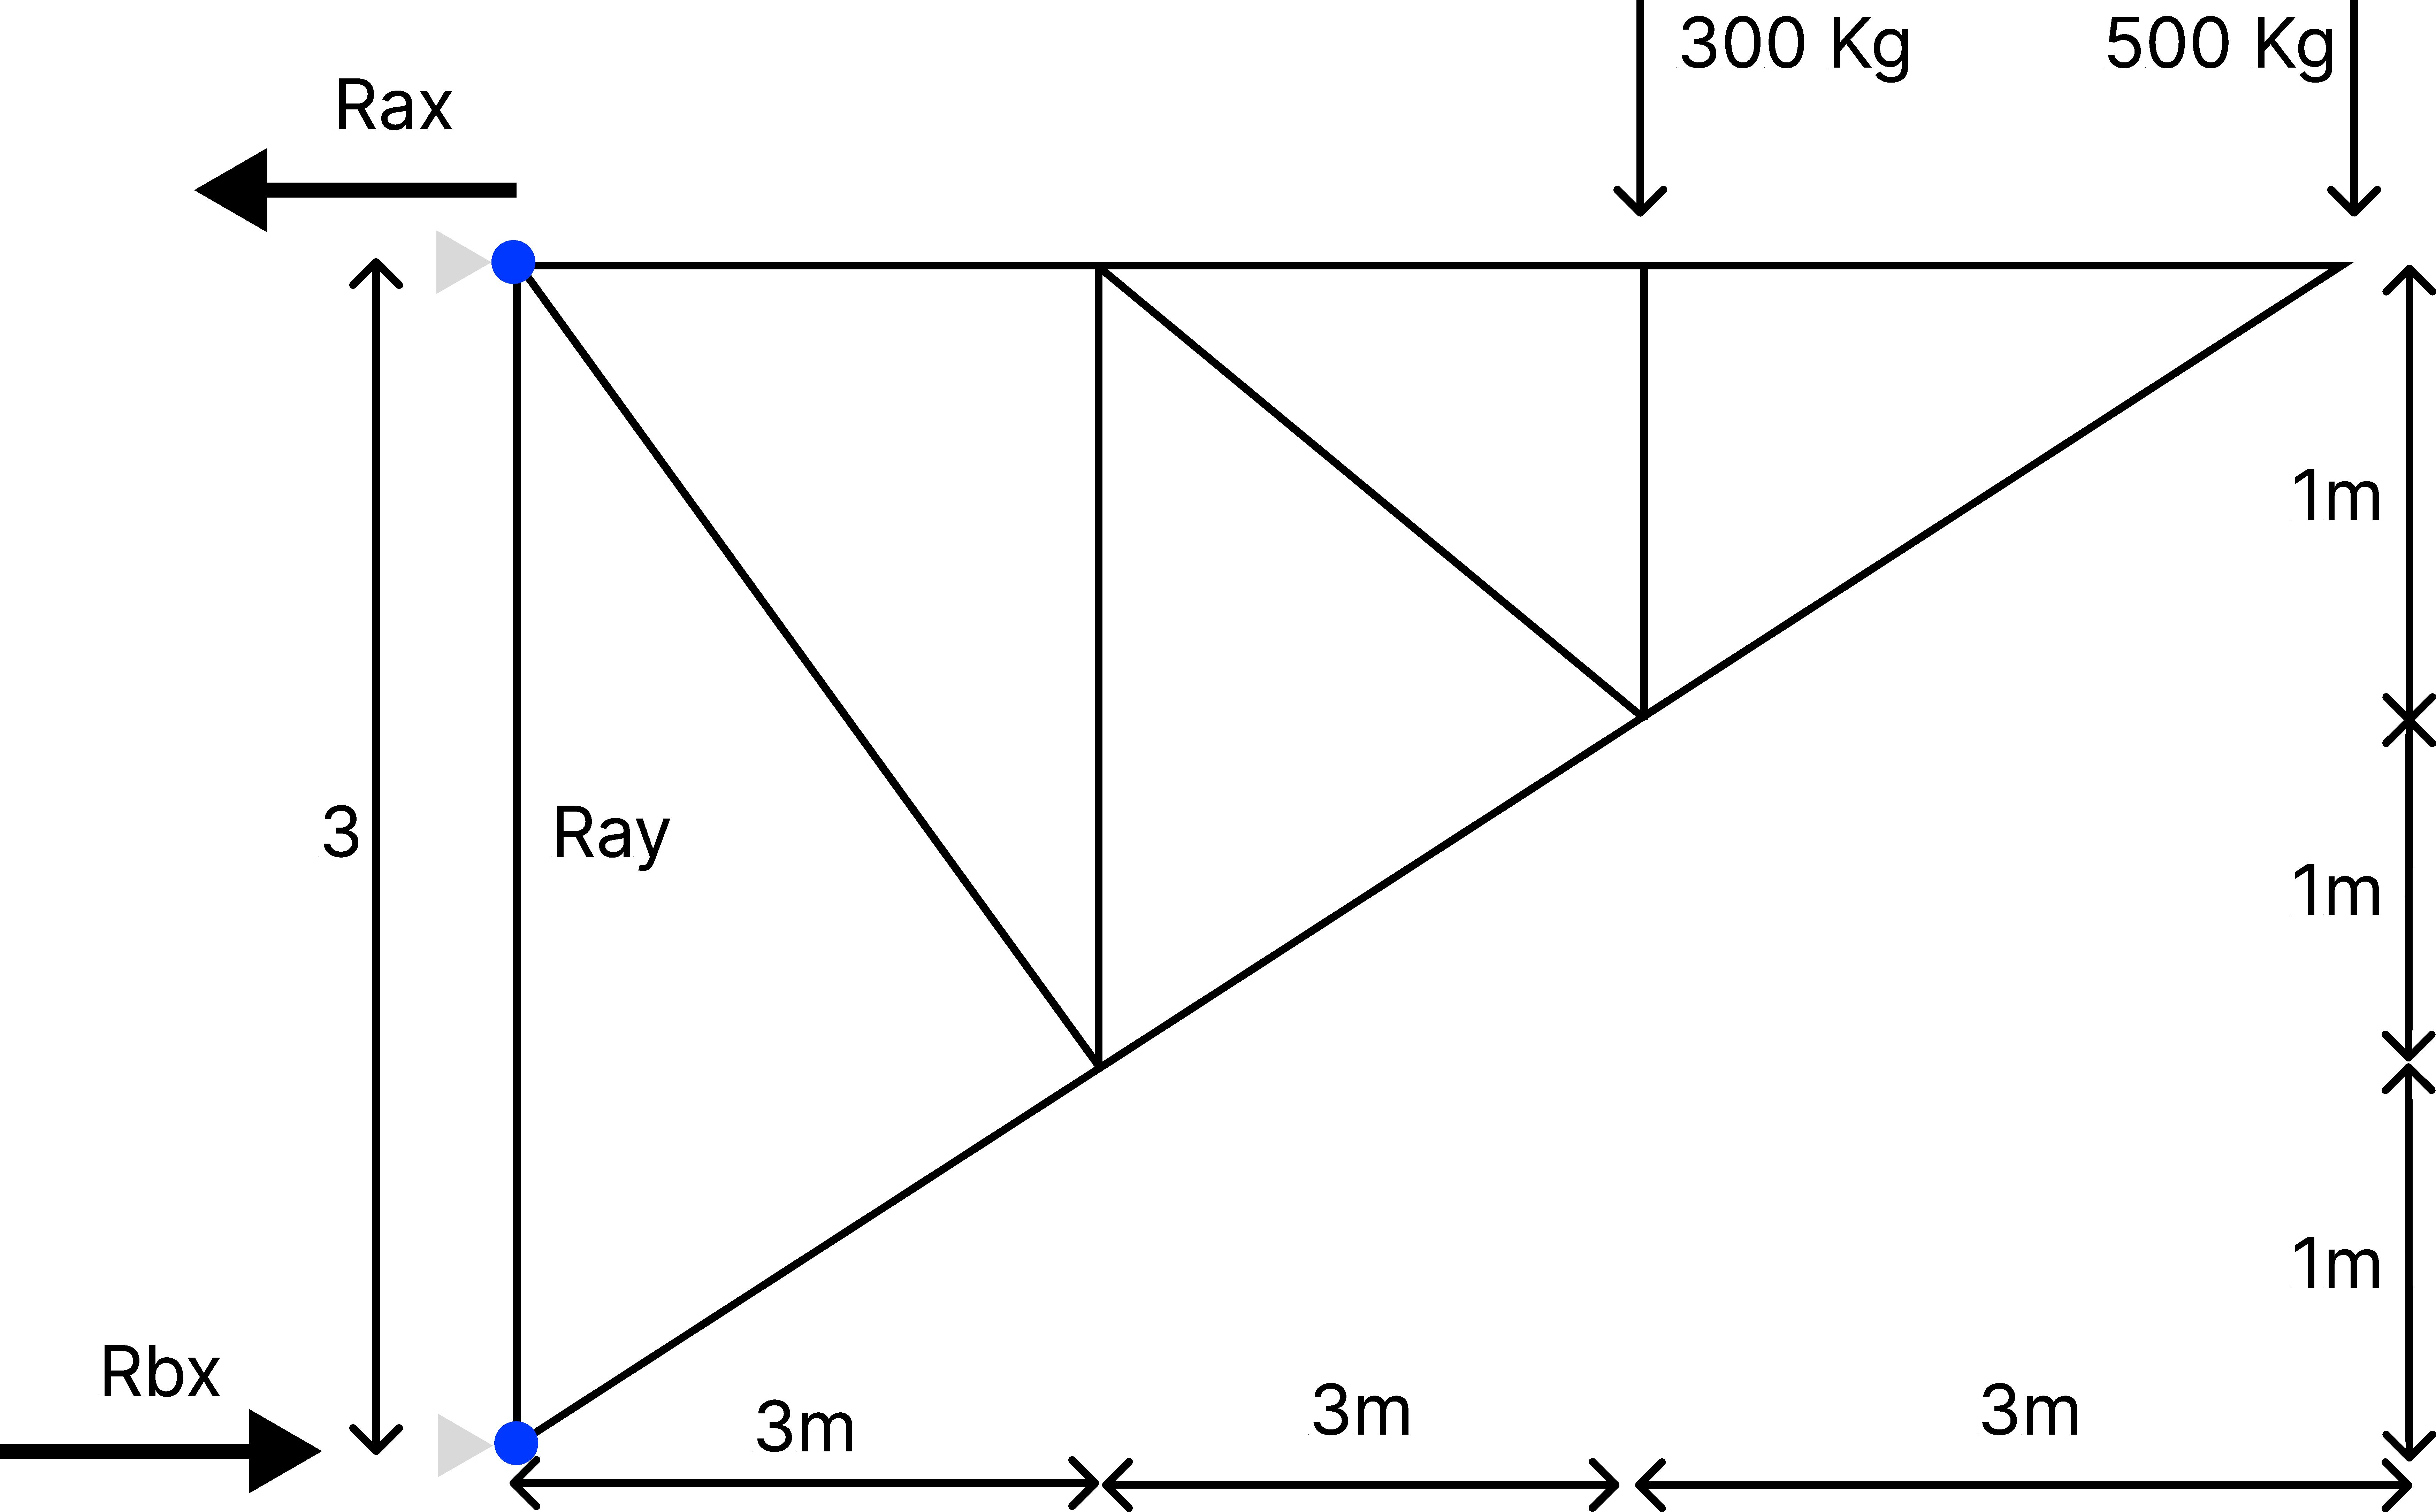
\includegraphics[width=0.5\textwidth]{emm1.pdf}
  \caption{Armadura simple e isostática}
  \label{emm1}
\end{figure}
\begin{align*}
    &\sum F_y = 0\\
    &R_{ AY} - 300 - 500 < 0\\
    &R_{AY} = 800kg\\
    &\sum M_A = 0; \circlearrowleft +\\
    &- 300(b) - 500(g) + R_{bx}(3) = 0 \\
    &R_{BX} = \frac{1800 + 4500 }{3} = 2100Kg_{f}
    &\sum F_x = 0\\
    &2100 - R_x = 0\\
    & R_{AX} =
\end{align*}
\begin{figure}[h!]
\centering
  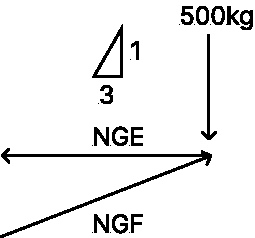
\includegraphics[width=0.5\textwidth]{emm2.pdf}
  \caption{Nodo g}
  \label{emm2}
\end{figure}
\begin{align*}
    &\sum F_y = 0; \uparrow +\\
    &- 500 + N_{FG}\left(\frac{1}{\sqrt{10}}\right) = 0\\
    &N_{FG} = \frac{500 \sqrt{10}}{1} = 0\\
    &\sum F_x = 0\\
    &- N_{GE} + 500 \sqrt{10}\frac{3}{\sqrt{10}}  =  0 \\
    & N_{GE} = 1500 Kg_f
\end{align*}



\begin{figure}[h!]
  \centering
    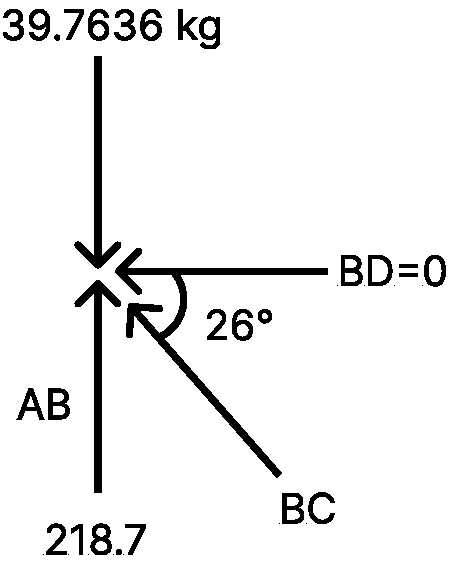
\includegraphics[width=0.5\textwidth]{emm3.pdf}
    \caption{Primer nodo}
    \label{emm3}
  \end{figure}
\begin{align*}
  &\sum F_y = 0\\
  &- 39.7636 + 218.7 \downarrow B\left(\sin{26} \right) = 0\\
  &Bc = - 408.1847\, Compresion\\
  &\sum F_x = 0\\
  &408.1847 \cos{26} - BD = 0\\
  &BD = 366.8789
\end{align*}
\begin{figure}[h!]
\centering
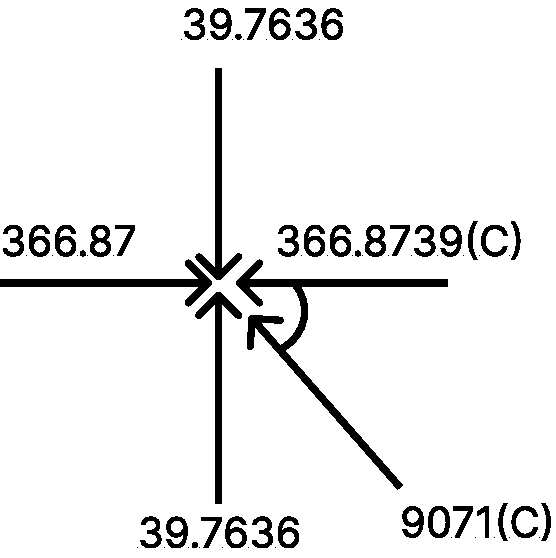
\includegraphics[width=0.5\textwidth]{emm4.pdf}
\caption{Segundo nodo}
\label{emm4}
\end{figure}
\begin{figure}[h!]
\centering
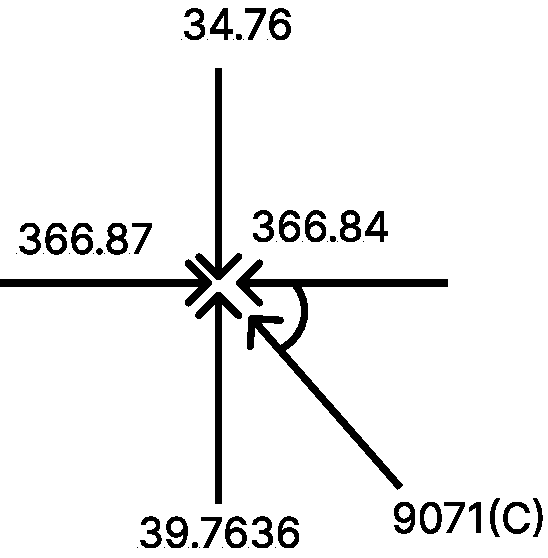
\includegraphics[width=0.5\textwidth]{emm5.pdf}
\caption{Tercer nodo}
\label{emm5}
\end{figure}
\begin{figure}[h!]
\centering
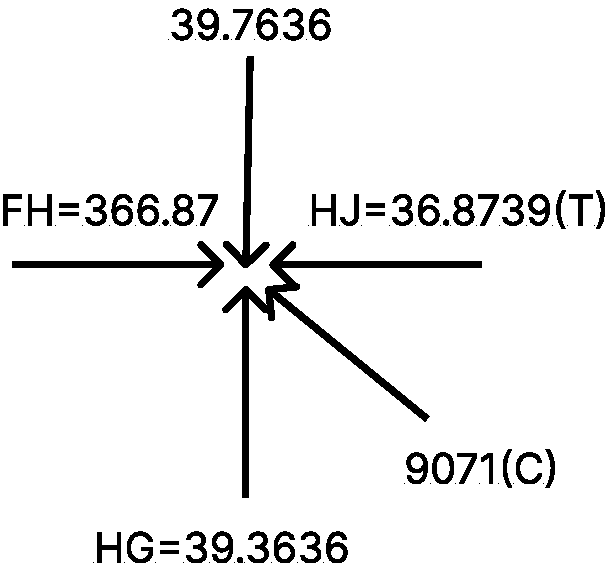
\includegraphics[width=0.5\textwidth]{emm6.pdf}
\caption{Cuarto nodo}
\label{emm6}
\end{figure}
\begin{figure}[h!]
\centering
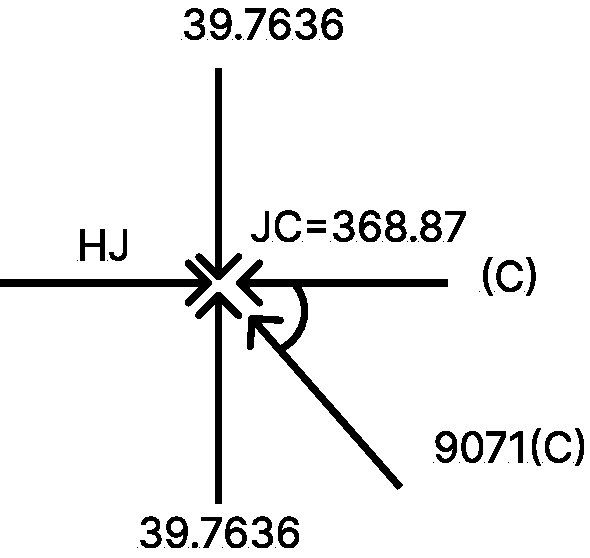
\includegraphics[width=0.5\textwidth]{emm7.pdf}
\caption{Quinto nodo}
\label{emm7}
\end{figure}
\begin{figure}[h!]
\centering
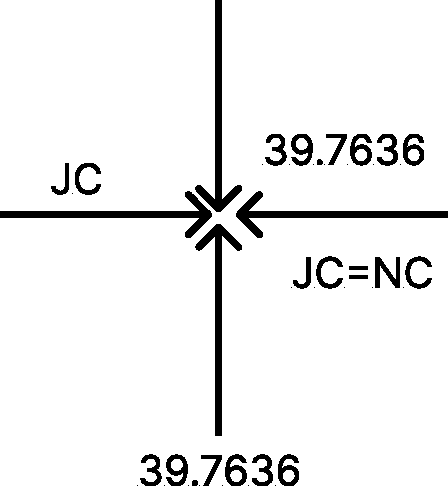
\includegraphics[width=0.5\textwidth]{emm8.pdf}
\caption{Sexto nodo}
\label{emm8}
\end{figure}
\begin{figure}[h!]
\centering
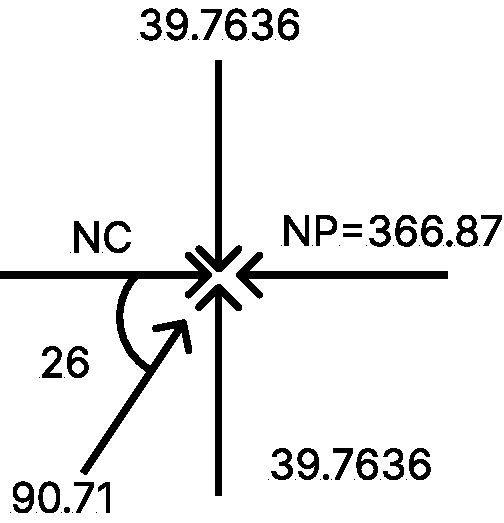
\includegraphics[width=0.5\textwidth]{emm9.pdf}
\caption{Séptimo nodo}
\label{emm9}
\end{figure}
\begin{figure}[h!]
\centering
\includegraphics[width=0.5\textwidth]{emm10.pdf}
\caption{Octavo nodo}
\label{emm10}
\end{figure}
\begin{figure}[h!]
\centering
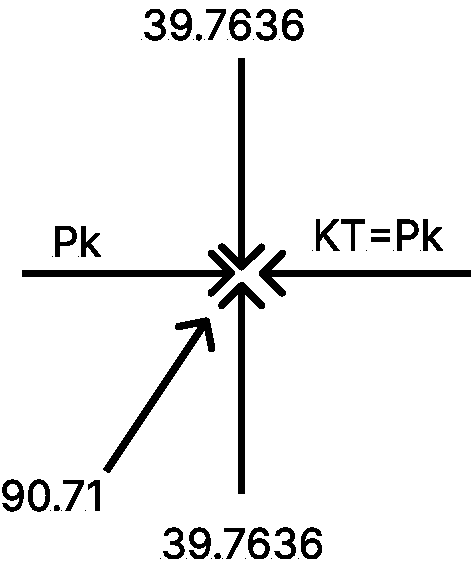
\includegraphics[width=0.5\textwidth]{emm11.pdf}
\caption{Noveno nodo}
\label{emm11}
\end{figure}
\begin{figure}[h!]
\centering
\includegraphics[width=0.5\textwidth]{emm12.pdf}
\caption{Décimo nodo}
\label{emm12}
\end{figure}
\begin{figure}[h!]
\centering
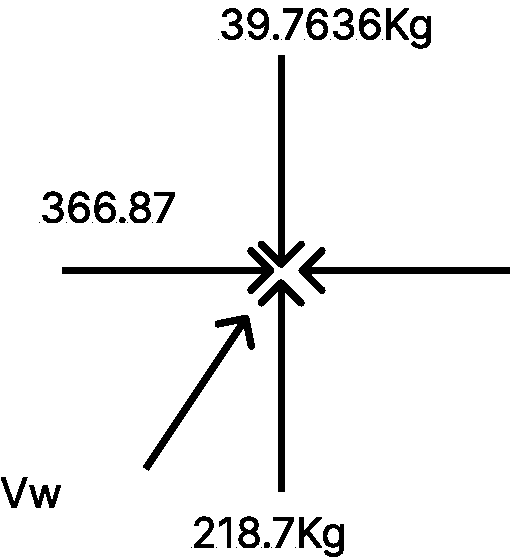
\includegraphics[width=0.5\textwidth]{emm13.pdf}
\caption{Décimo primer nodo}
\label{emm13}
\end{figure}
\begin{align*}
  &\sum F_y = 0\\
  &- 39.7630 + 218.7 + V_w \sin{26} = 0\\
  &V_w = - 408.1847 Kg\, (Compresion)
\end{align*}
\subsubsection{Tensión}
Excepto para miembros conectados con pasadores,$F_t$ no excederá de $0.60F_y$ en el área total, ni de $0.5F_u$ en el área neta efectiva\dots

Para miembros conectados con pasadores: $F_t= 0.45F_y$ en el área neta.
\begin{align*}
  &\sigma_t = 0.6F_y&& \text{Sección Masiza}\\
  &\sigma_t = 0.55F_y&& \text{Sección con orificios}
\end{align*}
\begin{figure}[h!]
\centering
  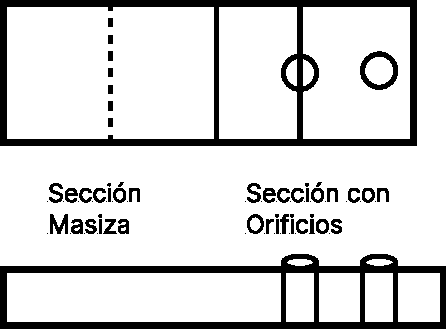
\includegraphics[width=0.5\textwidth]{emm15.pdf}
  \caption{Fuerzas de Tensión}
  \label{emm15}
\end{figure}
Lo cual, puede ser mejor visualizada en la figura \ref{emm16}
\begin{figure}[h!]
\centering
  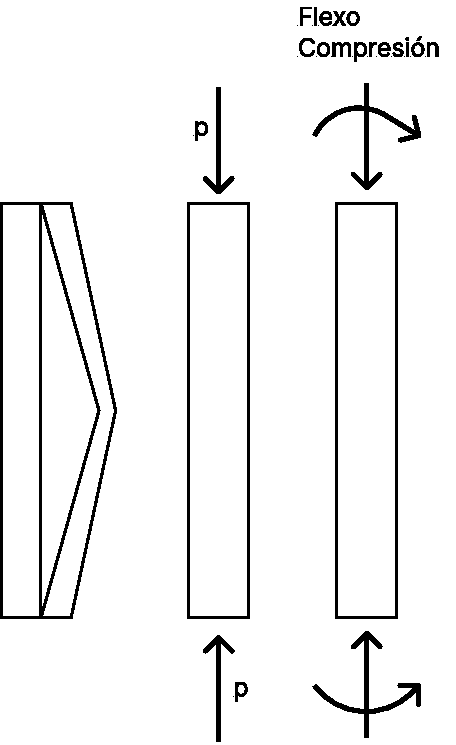
\includegraphics[width=0.5\textwidth]{emm16.pdf}
  \caption{Formas de compresión de P}
  \label{emm16}
\end{figure}
\begin{notation}
  \begin{itemize}
    \item $K=$ Factor de restricción en el extremo del elemento
    \item $l=$ Longitud física
    \item $L_e= Kl=$ Longitud efectiva
  \end{itemize}
\end{notation}
La esbeltez, es igual a:
\begin{equation}
  \frac{kl}{r}
\end{equation}
\begin{equation}
  r = \sqrt{\frac{I}{A}}
\end{equation}
\subsubsection{Cortante}
En el área efectiva de la sección transversal que resiste el esfuerzo cortante:
\begin{equation}
  F_v = 0.4F_y
\end{equation}
En perfiles laminados y en perfiles armados, el área efectiva para resistir cortante podrá calcularse como el producto del peralte total por el espesor del alma.

En las conexiones de extremo de vigas, donde el patín superior esté cortado y en situaciones similares donde puede ocurrir falla por cortante a lo largo de un plano que pase a través de los sujetadores, o por una combinación de cortante a lo largo de un plano que pase a través de los conectores, más tensión a lo largo de un plano perpendicular, en el área efectiva para resistir falla por desgarramiento:
\begin{equation}
  F_v = 0.3F_u
\end{equation}
\subsubsection{Compresión}
En la sección total de miembros cargados en compresión axial, cuya sección transversal cumple con las disposiciones, cuando $Kl/r$, la mayor relación de esbeltez efectiva de cualquier segmento no arriostrado como se define, es menor que $C_r$:
\begin{equation}
  F_a = \frac{\left[1 - \frac{\left(\frac{Kl}{r}\right)^2}{2C_c^2} \right]F_y}{ \frac{5}{3} + \frac{3\left(\frac{Kl}{r}\right)^3}{8C_r} }
\end{equation}
en donde:
\begin{equation}
  C_c = \sqrt{\frac{2\pi E}{F_y}} 
\end{equation}
En la sección total de miembros en compresión axial, cuando $Kl/r$ excede $C_c$
\begin{equation}
  F_a = \frac{12 \pi^2 E}{23\left(\frac{Kl}{r}\right)^2}
\end{equation}
\subsection{Determinación de la presión de diseño}

\begin{equation}
    \text{Presión} = 0.048 Cp V^2/n
\end{equation}
\begin{notation}
    \begin{itemize}
        \item $C_p=$ Depende de la forma del objeto que se opone al flujo del viento 
        \item $V_D=$ Velocidad de diseño
    \end{itemize}
\end{notation}
\subsubsection{Determinación de la velocidad de diseño}
Los efectos estáticos del viento sobre una estructura o componente de la misma, se determinan con base en la velocidad de diseño. Dicha velocidad de diseño se obtendrá de acuerdo con la ecuación \eqref{eqemm1}:
\begin{equation}
    V_D = F_{TR} D_{\alpha}V_R
    \label{eqemm1}
\end{equation}
\begin{notation}
    \begin{itemize}
        \item $F_{TR}=$ Factor  correctivo que toma en cuenta las condiciones locales relativas a la topografía u a la rugosidad del terreno en los alrededores del sitio de desplante
        \item $F_{\alpha}=$ Factor que toma enc uenta la variación de la velocidad ocn la altura $y$
        \item $V_R=$ Velocidad regional según la zona que le corresponde al sitio en donde se construirá la estructura.
    \end{itemize}
\end{notation}

\subsubsection{Factor de Exposición}
El coeficiente $F_{\alpha}$ refleja la variación de la velocidad del viento con respecto a la altura Z. Asimismo, considera el tamaño de la construcción o de los elementos de recubrimiento y las características de exposición.
El factor de exposición se calcula con la siguiente expresión:
\begin{equation}
    F_{\alpha}= F_C F_{rz}
\end{equation}

\begin{notation}
    \begin{itemize}
        \item $F_C$ Es el factor que determina la influencia del tamaño de la construcción, adimensional, y
    \item $F_{rz}$ El factor que establece la variación de la velocidad del viento con la altura Z en función de la rugosidad del terreno de los alrededores, adimensional. 
    \end{itemize}
\end{notation}

\subsubsection{Factor de tamaño}
El Factor de Tamaño, $F_C$ es el que toma en cuenta el tiempo en el que la ráfaga del viento actúa de manera efectiva sobre una construcción de dimensiones dadas. Considerando la clasificación de las estructuras según su tamaño
\begin{table}[h!]
    \centering
    \begin{tabular}{@{}cc@{}}
    \toprule
    CLASE DE ESTRUCTURA & $F_C$   \\ \midrule
    A                   & 1.00 \\
    B                   & 0.95 \\
    C                   & 0.90 \\ \bottomrule
    \end{tabular}
    \caption{ Factor de tamaño, $F_C$}
    \label{tabemm}
\end{table}
\subsubsection{Factor de rugosidad y altura}
El factor de rugosidad y altura, $F_{rz}$, establece la variación de la
velocidad del viento con la altura Z. Dicha variación está en
función de la categoría del terreno y del tamaño de la
construcción.
Se obtiene de acuerdo con las expresiones siguientes:
\begin{align*}
F_{rz} = 1.56 \left(\frac{10}{\sigma}\right)^{\alpha}&& \text{si } Z\leq 10\\
F_{rz} = 1.56 \left(\frac{Z}{\sigma}\right)^{\alpha}&& \text{si } 10 < Z < \sigma\\
F_{rz} = 1.56 && \text{si } Z\leq \sigma
\end{align*}
\begin{notation}
    \begin{itemize}
        \item $\sigma$ Es la altura, medida a partir del nivel del terreno de desplante, por encima de la cual la variación de la velocidad del viento no es importante y se puede suponer constante; a esta altura se le conoce como altura gradiente; $\sigma$ y Z están dadas en metros, y
        \item $\alpha$ Exponente que determina la forma de la variación de la velocidad del viento con la altura y es adimensional.
    \end{itemize}
\end{notation}